\documentclass[handout]{beamer}
%\documentclass[xcolor=pst]{beamer}
%\usepackage[spanish]{babel}
\usepackage[utf8]{inputenc}

\usepackage{amssymb,amsmath}
\usepackage{graphicx}
%\usepackage[pdf]{pstricks}
\usepackage{colortbl}
\definecolor{fucsia}{rgb}{1,0,1}
%\usepackage[Q=yes]{examplep}

\newcounter{savedenum}
\newcommand*{\saveenum}{\setcounter{savedenum}{\theenumi}}
\newcommand*{\resume}{\setcounter{enumi}{\thesavedenum}}

%\usepackage{default}
\usetheme{Madrid}

%\setbeamertemplate{caption}[numbered]


\title[L-Shape Selection]{A heuristic algorithm to select genes potentially regulated by methylation}
\author[Álex Sánchez]{Alex Sánchez, Berta Mir\'o, Francesc Carmona, \\
	Sarah Bazzoco and Diego Arango del Corro}
\date[]{July 09, 2018}

\begin{document}
\begin{frame}
	
\begin{scriptsize}
\begin{center}
  \emph{ XXII International Biometric Conference}
\end{center}
\end{scriptsize}

\titlepage

\begin{columns}
   \column{0.7\textwidth}
   \scriptsize
   Genetics, Microbiology and Statistics Department \\ 
   \textbf{Facultad de Biología, Universitat de Barcelona}\\
   Statistics and Bioinformatics Unit (UEB)\\
   Department Molecular Oncology-CIBBIM \\ 
   \textbf{Vall Hebron Institut de Recerca}

  \hfill\column{0.3\textwidth}
  
\includegraphics[height=1cm]{images/alllogos.png}
% 
\includegraphics[height=0.5cm]{images/VHIR_fonstransp.png}
\end{columns}

\end{frame}


\begin{frame}
\frametitle{Table of Contents}
\tableofcontents
\end{frame}

\section{Motivation}

\subsection{Genome-wide analysis of colorectal cancer}

\begin{frame}{Genome-wide analysis of colorectal cancer}
  \begin{itemize}
  \item This study originates in a work aiming at the identification of biomarkers for chemotherapy sensitivity in colorectal cancer (CRC) where the number of available therapies is smaller than in other cancer types.
  \item The study analyzed a panel of 30--45 cell lines derived from colorectal tumors characterized by increasing sensitivity to several chemotherapy drugs such as \begin{itemize}
                \item Irinotecan,
                \item Cetuximab,
                \item Oxaliplatin.
              \end{itemize}
  \end{itemize}
\end{frame}

%\subsection{The data}
\begin{frame}{Data for the study}
  \begin{itemize}
     \item Different high-throughput data were generated:
     \begin{itemize}
       \item gene expression from Affymetrix (HGU133p2) microarrays,
       \item microRNAs from Affymetrix miRNA array,
       \item methylation, from Illumina Beadchips,
       \item Copy Number Variation from Affymetrix Chip,
       \item \emph{RNA-seq data}
     \end{itemize}

    \item In this work we focus on one of the branches of the work: \\
        \textbf{\emph{the search of genes regulated by methylation}}.
  \end{itemize}
\end{frame}

%\subsection{Preliminaries}

\begin{frame}[fragile]\frametitle{Methylation}
\begin{itemize}
\item Methylation of CpG dinucleotides in the promoter of genes
  involved in the oncogenic process has been shown to be a key process
  contributing to tumor initiation and/or progression.
\item Essentially (and especially in cancer) methylation acts by inhibiting gene expression that
  is,\emph{ the more methylated is a gene the more repressed is its expression}
\begin{center}
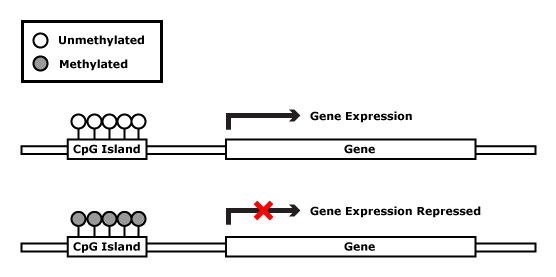
\includegraphics[width=0.7\textwidth]{./images/methylationAction1.png}
\end{center}
%\item Methylation is seen however as a dual phenomenon\\
%\label{sec-1.8.3}
%\begin{itemize}
%\item A methylated gene is "off"\\
%\label{sec-1.8.3.1}
%\item An unmethlated gene is "on"\\
%\label{sec-1.8.3.2}
%\end{itemize} % ends low level
%\item So in practice an important practical problem is to determine at which methylation level a gene is seen as "methylated" (that is turned off).\\
%\label{sec-1.8.4}
\end{itemize}
\end{frame}


\begin{frame}[fragile]\frametitle{Data are not univocally related}
\begin{center}
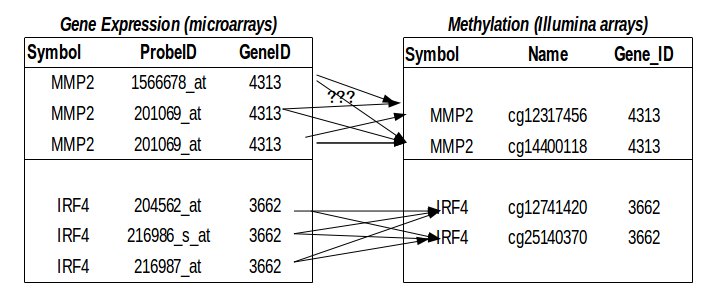
\includegraphics[width=0.9\textwidth]{./images/methSitesVSexprSites.png}
\end{center}

\end{frame}

\begin{frame}[fragile]\frametitle{Methylation and gene expression}
\begin{itemize}
\item Although the relation between methylation and gene expression is probably continuous ("\emph{the more...the less...}"),
\begin{center}
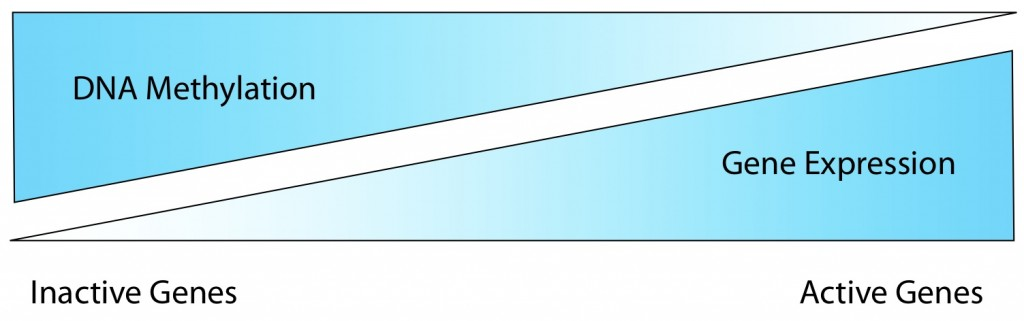
\includegraphics[width=0.7\textwidth]{./images/DNA-Methylation-and-Gene-Expression-Relationship.jpg}
\end{center}
\item methylation is, in practice, seen as a dual phenomenon
\begin{itemize}
\item A methylated gene is ``off''
\item An unmethylated gene is ``on''
\end{itemize}
\item Practical problem: \textbf{\emph{at which methylation level a gene is seen as ``methylated'' (is it ``turned off'')?}}
\end{itemize}

\end{frame}


\begin{frame}{Patterns of (negative) association}
  \begin{itemize}
  \item Considering the relation between methylation and expression in cancer (the higher methylation the lower the expression...)
\item leads to expecting that scatterplots depicting the relation between methylation and expression show a negative correlation.
\item This is so and indeed genes known to be regulated by methylation use to show an L-shape pattern in these plots.
  \end{itemize}
\begin{center}
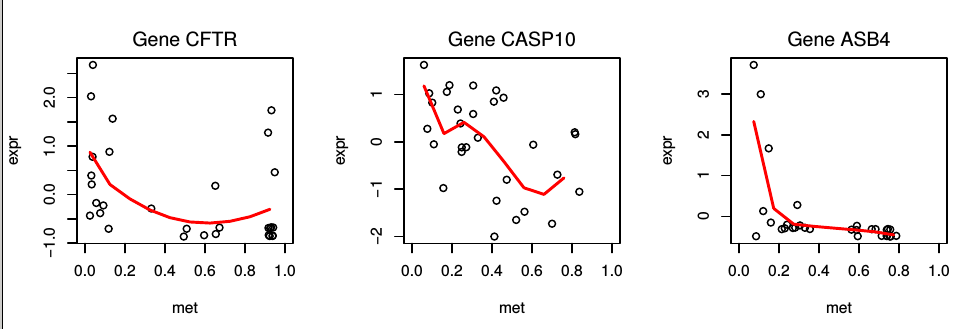
\includegraphics[width=0.7\textwidth]{./images/Lshapes1.png}
\end{center}
\end{frame}

\begin{frame}{Selecting genes by mining scatterplots}
  \begin{itemize}
  \item Assuming the relation described above is true...
\item Finding genes regulated by methylation is equivalent to finding genes whose methylation--expression scatterplot has an L--shape.
\item There is a scatterplot \emph{per} gene and thousands of genes:\\ \textbf{\emph{An automatic method for selecting interesting genes through their scatterplots is required}}.
  \end{itemize}
\end{frame}


\subsection{Objectives}

\begin{frame}[fragile]\frametitle{Objectives}
The main objectives of this work are:
\begin{enumerate}

\item To introduce a new method to select genes showing an L-shape
\item To compare it with previously available methods, 
\item To apply the selected methods on a specific CRC dataset and validate the findings based on their biological relevance.

\end{enumerate}

\end{frame}

\section{Methods for selecting L--shaped patterns}

\begin{frame}{Overview of approaches}
\begin{itemize}
\item We have investigated three approaches for selecting L--shaped patterns in scatterplots
\begin{enumerate}
\item Use Conditional Mutual Information to detect threshold point and select genes.
\item Clustering scatterplots based on the results of Splines Regression and select L-shape clusters.
\item \emph{Apply Functional Data Analysis techniques to estimate shapes and cluster to extract L--paterns.}
\end{enumerate}
\item Only the first two have provided interesting results so the third is omitted.
\end{itemize}
\end{frame}


\subsection{Selection based on conditional mutual information}

\begin{frame}%[allowframebreaks]
\frametitle{Selection based on conditional mutual information}
This method was originally proposed by Liu (2012) to study a huge (hundreds of multi--cancer samples) TCGA dataset.\\
Assume
 \begin{itemize}
  \item That the genes we want to select show an L--shape pattern.
\item That methylation is \emph{truly binary}
\end{itemize}
This has two implications:
\begin{itemize}
\item The reflection point of the L-shape is an appropriate choice to
  binarize methylation data % \footnote{That is values on the left of this point can be considered to be methylated and values on the right can be considered to be unmethylated},
and
\item Conditioning on the binarized on-off methylation status, the
  continuous valued methylation data and expression data should be
  independent% \footnote{That is both branches of the ``L'' pattern show many differenta wide range of values of methylation (left) or expression (right) for a small range of values of expression (left) or methylation (right) which suggest that once we are on one or other side of the binarization point methylation and expression are independent}.
\end{itemize}
\end{frame}

\begin{frame}{Data binarization}
\begin{itemize}
\item A relevant issue is how the continuous methylation data are binarized.
\item Liu (2012) suggested to use different thresholds,\\
 and select the threshold that best separated the two regions.
\item The ``best'' criteria is based on computing mutual information.
\end{itemize}

\end{frame}



\begin{frame}[allowframebreaks]
\frametitle{Mutual Information and Conditional Mutual Information}
\begin{itemize}
\item   \emph{Mutual Information} between two random variables $X$
and $Y$ measures the information that these variables share.
% it measures how much knowing one of these variables reduces uncertainty about the other.
\item For discrete variables it is defined as:
\[
 I(X;Y)= \sum_{y \in Y} \sum_{x \in X}
                 p(x,y) \log{ \left(\frac{p(x,y)}{p(x)\,p(y)}
                              \right) }, \,\!
\]
%where $p(x,y)$ is the joint probability distribution function of $X$ and $Y$, and $p(x)$ and $p(y)$ are the marginal probability distribution functions of $X$ and $Y$ respectively.
\item Knowledge of a third variable, $Z$, can increase or decrease the mutal
information between $X$ and $Y$.
\item \emph{Conditional Mutual Information} is the expected value of $I(X;Y)$ once $Z$ is
known.
\[
I(X;Y|Z) = \mathbb E_Z \big[ I(X;Y)|Z\big ]
\]
% \begin{eqnarray*}
% I(X;Y|Z) &=& \mathbb E_Z \big(I(X;Y)|Z\big) \\
%    &=& \sum_{z\in Z} p_Z(z) \sum_{y\in Y} \sum_{x\in X}
%      p_{X,Y|Z}(x,y|z) \log \frac{p_{X,Y|Z}(x,y|z)}{p_{X|Z}(x|z)p_{Y|Z}(y|z)},
% \end{eqnarray*}
\end{itemize}

\framebreak

\begin{block}{The key idea}
To determine whether methylation and expression of a gene exhibit an L-shape,
one can compute the conditional Mutual Information (MI) for different choices of threshold
to binarize the methylation data.
\end{block}
If we consider the continuous valued methylation and expression data as two random variables
$X$ and $Y$, and denote a nominal threshold as $t$, the conditional MI can be written as a
weighted sum of MIs on the two sides of the threshold.
\[
\mathit{cMI}(t)=I(X,Y|X>t) P(X>t) + I(X,Y|X\le t)P(X\le t)
\]
\end{frame}
%\framebreak

\begin{frame} {cMI for L--shaped genes}
\begin{itemize}
\item When $t$ is $0$ or $1$, $\mathit{cMI}$ equals to the mutual information derived
from all data points, so, for an L--shaped gene i is verified that:
\item
as $t$ moves from 0 to 1, $\mathit{cMI}(t)$ first decreases and then
increases, and its value approaches zero when $t$ coincides with the reflection point.
%\item The ratio $r=\frac{\min\{\mathit{cMI}(t)\}}{\mathit{cMI}(0)}$ for an L-shape gene is small,
\end{itemize}

\begin{center}
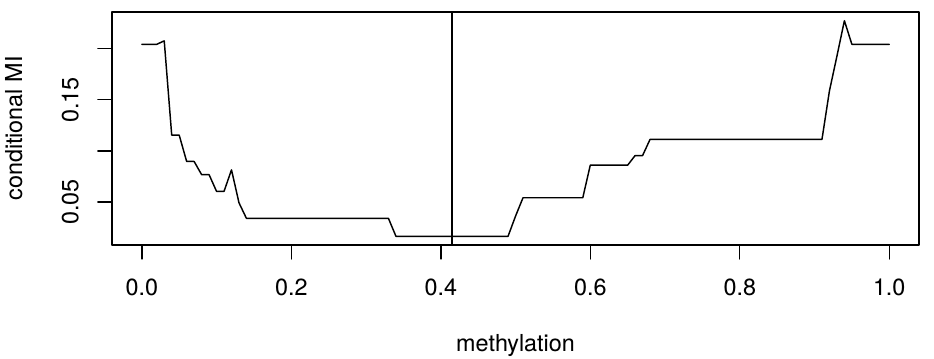
\includegraphics[height=3cm]{./images/cMI-methylation.png}
\end{center}
\end{frame}


\begin{frame} {Optimal threshold for binarizing methylation data}
The behavior of cMI(t) for an L-shape gene, suggests the following criteria to select the optimal binarization point
\begin{block}{Optimal threshold}
$t^{\ast} = \mathrm{argmin}\{ \mathit{cMI}(t) \}$ is the optimal threshold for
dichotomizing the methylation data of this gene.
\end{block}
L-shape genes will be selected as those verifying reasonable conditions such as:
\begin{enumerate}
\item $r=\frac{\min\{\mathit{cMI}(t)\}}{\mathit{cMI}(0)}$ is ``small enough''.
\item Minimum value of unconditioned MI $\mathit{cMI}(0)$ is ``big enough''.
\item Left side of the graph reaches higher values than right side
\end{enumerate}

\end{frame}

%\begin{frame}{Joint distribution estimator}
%To estimate the MI terms we use a kernel-based estimator, which %constructs a joint
%probability distribution by applying a Gaussian kernel to each %data point, and estimates
%the MI based on the joint distribution. The estimator is as %follows:
%\[
%I(X,Y) = \frac 1M \sum_{i=1}^M \log\frac{M\sum_{j=1}^M %e^{-\frac{1}{2h^2}((x_i-x_j)^2+(y_i-y_j)^2)}}{%
%                                      \sum_{j=1}^M %e^{-\frac{1}{2h^2}(x_i-x_j)^2} \sum_{j=1}^M %e^{-\frac{1}{2h^2}(y_i-y_j)^2}}
%\]
%where $h$ is a tuning parameter for the kernel width and %empirically set $h=0.3$.
% i and j are indices for samples.
% In our analysis, we normalize the expression data to zero %mean.
%\end{frame}

\subsection{Selection based on Spline regression}

\begin{frame}{Spline Regression}
\begin{itemize}

\item Regression based on splines (Hastie et al. 2009) is a form of non-parametric
  regression that automatically models non-linearities and
  interactions between variables.
\item This is done using \emph{Splines},  continuous functions formed by connecting linear
segments. \\ The points where the segments connect are called the \emph{knots} of the spline.
\item A particularly efficient form of splines regression is  $B$-splines where the splines are  $B_{mp}$ $p$-th order polynomial of degree $p-1$ with finite support over the interval and 0 everywhere.
    
%\begin {itemize}
%\item $\varsigma=\lbrace t_1 < \cdots < t_N \rbrace$ non decreasing  knot sequence
%\item $\left[ t_m,t_{m+1} \right)$ half open interval
%\item $B_{mp}$ $p$-th order polynomial (degree $p-1$) with finite support over the interval and 0 everywhere else so that  $\sum_{m=1}^{N-p}B_{mp}(x)=1$
%\item then  $s(x)=\sum_{m=1}^{N-p}B_{mp}(x)c_m$
%\end{itemize}
\end{itemize}
\end{frame}

%\begin{frame}{Clustering using Spline regression}
%To represent the curve we set:
%\[
%y_{ij}=s(x_{ij})
%\]
%So
%\[
%\mathbf{y}_i=\mathbf{B}_i\mathbf{c}
%\]
%with
%\begin {itemize}
%\item $\mathbf{B}_i=\left[ B_{1p}\mathbf{x}_i,B_{2p}\mathbf{x}_i,\dots,B_{Lp}\mathbf{x}_i \right]$ the spline basis matrix
%\item $\mathbf{c}$ the vector of spline coefficients.
%\end{itemize}
%\end{frame}

\begin{frame}{Clustering using Spline regression}
Algorithm
\begin {enumerate}
\item Select of the genes with a negative significant correlation.
    \\ Eventually apply heuristic additional filters that removes genes that are clearly non-L-shaped.
\item Fit a cubic regression splines curve to each pair expression--methylation.
\item Cluster the resulting splines coefficients
\item Select genes in clusters that correspond to L--shapes
\end{enumerate}
\end{frame}

\section{Results}

%\begin{frame}{Algorithm for combining both methods}

%\end{frame}

\subsection{Results from using cMI to select genes}
\begin{frame}{Results (1) Conditional Mutual Information}
\begin {itemize}
\item Data: Expression and Methylation values from 30 cell lines: two 30 $\times$ 11746 arrays.
\item No previous filtering of the genes was needed/performed
%\begin{block}{Criteria used for selecting genes}
\item Tune L-shape selection using a combination of three criteria:
\begin{itemize}
\item Genes with ``small'' ratio  $r=cMI/MI <0.25$
\item Minimum value of unconditioned MI $\mathit{cMI}(0)>0.1$
\item Median expression on the left side of the optimal threshold $t^{\ast}$ must be higher
than median expression on the right side.
\end{itemize}
%\end{block}
\item Tuning values selected using cross-validation
\item % According to the above criteria,
\textbf{A total of 641 genes are selected to be L-shape genes}.
\end{itemize}
\end{frame}


\subsection{Results from using Splines regression to select genes}

\begin {frame}{Results (2) Splines--based regression}
\begin {itemize}
\item Using the same dataset we
\begin{enumerate}
  \item selected genes with significant negative spearman correlation
  \item applied additional filters to guarantee non L-shape removal.
\end{enumerate}
\item After the previous selection of genes we worked with 191 genes
\item A hierarchichal clustering yields 5 clearly defined clusters
\item The 2 first clusters included the genes with an L-shape
\end{itemize}
\begin{center}
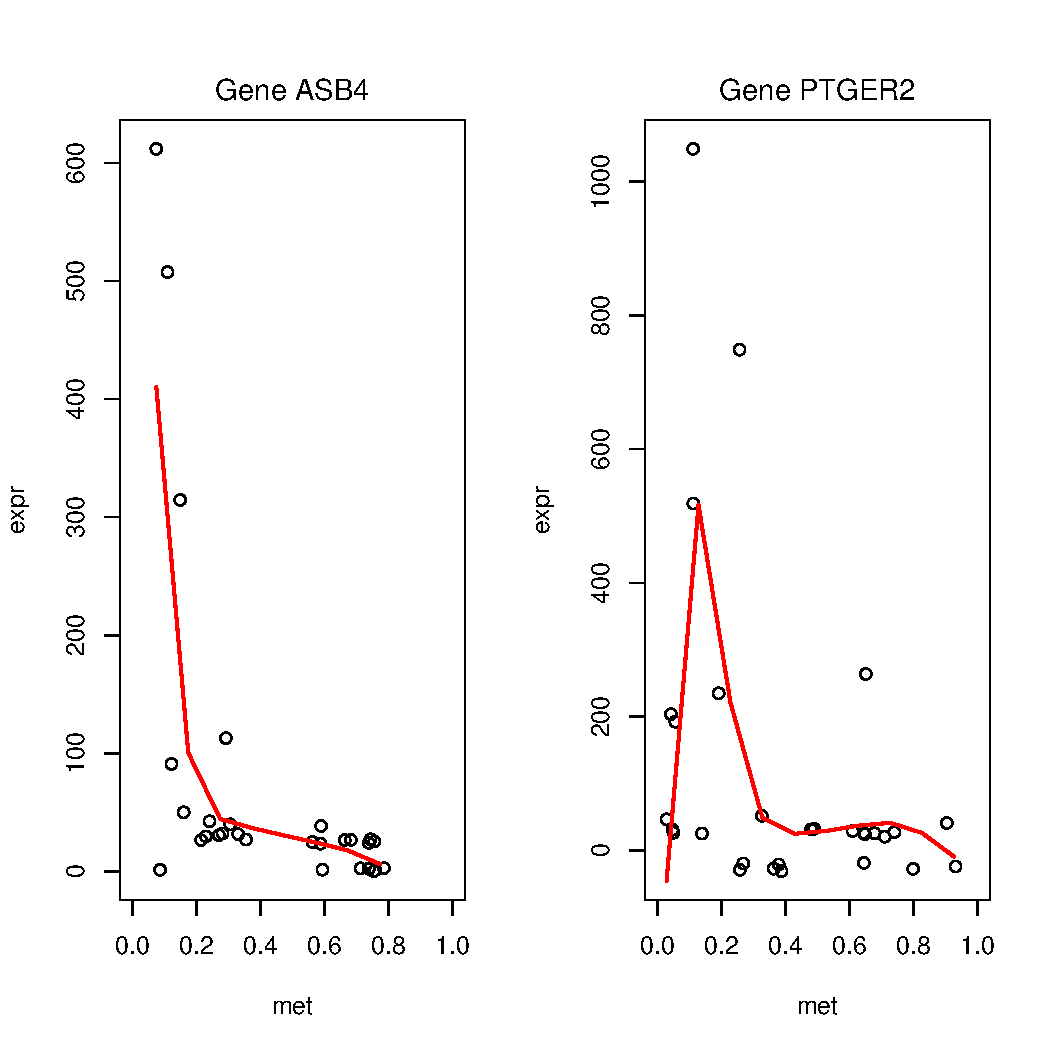
\includegraphics[height=4.5cm]{./images/grafic_two_patterns.pdf}
\end{center}
\end{frame}


\begin{frame}{Results (3)}
The results of both methods that can be summarized in the following table:
\begin{columns}
\begin{column}{.5\linewidth}
\begin{center}
\begin{tabular}{|c|c|c|}
\hline
Initial selection & 191 & 641 \\
\hline
\hline
Cluster & Splines & cMI \\
\hline
1 & 140 & 102 \\
2 & 22 & 16 \\
\hline
Total & 162 & 118 \\
\hline
\end{tabular}
\end{center}
\end{column}
\begin{column}{.5\linewidth}
\begin{center}
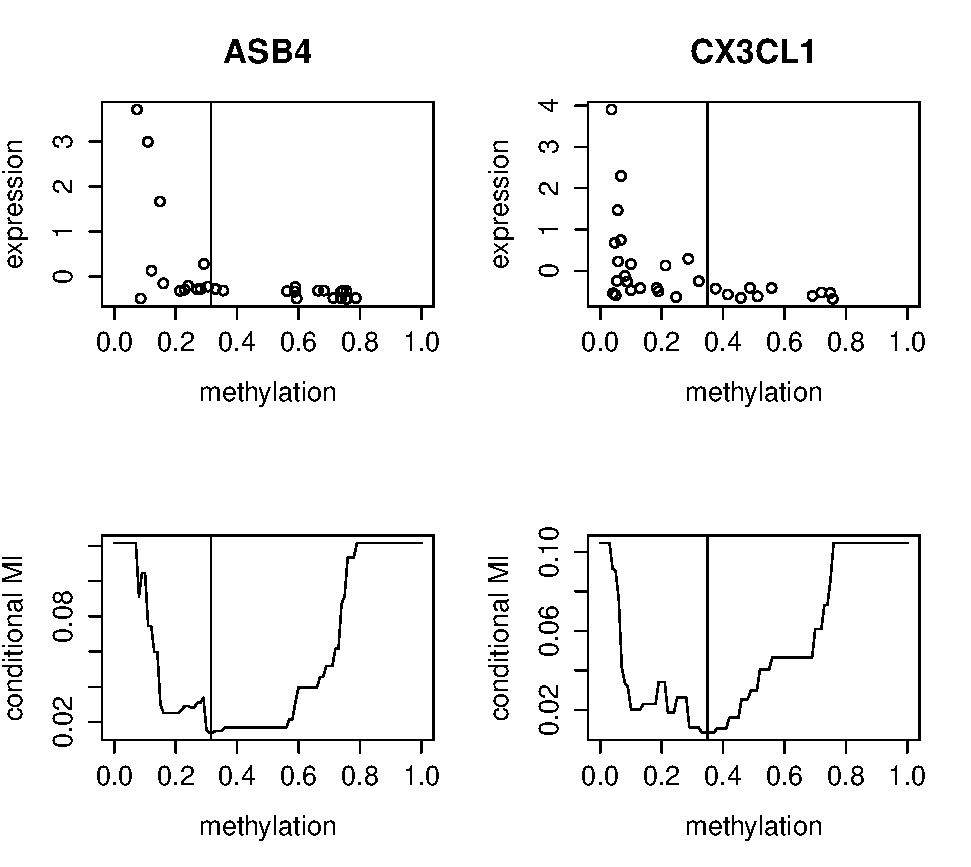
\includegraphics[height=5cm]{./images/grafic_two_genes.pdf}
\end{center}
\end{column}
\end{columns}
\end{frame}

%\begin{frame}{Biological significance assessment}

%\end{frame}

\section{Discussion and Conclusions}

\begin{frame}{Discussion and Conclusions}
  \begin{itemize}
  \item cMI based gene selection provides an intuitive approach for selecting L--shaped patterns although it can yield a certain number of "false positives".
  \begin{itemize}
         \item The method, however works well with big (hundreds) samples which makes it less reliable for normal-size (dozens) datasets.
  \end{itemize}
  \item Clustering based on the results of Splines regression is also useful in detecting L--shaped patterns.
       \begin{itemize}
         \item It selects a smaller number of genes than cMI,
         \item It is not so dependent from sample size
       \end{itemize}
  \item Biological interpretation is still ongoing but the results are consistent with the hypothesis
    (genes known to be regulated by methylation have been found with both methods).
\end{itemize}
\end{frame}

\section*{References}
\begin{frame}\frametitle{References}
\begin{thebibliography}{9}
%\addcontentsline{toc}{chapter}{\numberline{}Bibliografía}
%
%\bibitem{cohen} J. Cohen, \emph{Statistical power analysis for the behavioral sciences} (2nd ed.). % Hillsdale,NJ: Lawrence Erlbaum, 1988.

%\bibitem{faraway} J.J. Faraway, \emph{Linear Models with R}, Chapman \& Hall/CRC, 2004.

%\bibitem{montgomery} D.C Montgomery \emph{Design and Analysis of Experiments}, John Wiley \& Sons, 2008.

%\bibitem{blog} \texttt{http://erre-que-erre-paco.blogspot.com.es/2013/04/el-codigo-body-td-font-family-sans.html}

\bibitem{Bazzocco:2014} Bazzocco, S., Alazzouzi, H., Ruiz de Villa, M. C., Sanchez-Pla, A., Mariadason, J.M., Arango D. (2014) \emph{Genome-Wide Analysis of DNA Methylation in Colorectal Cancer}. Submitted.

\bibitem{Hastie:2009} Hastie T., Tibshirani R., and Friedman J.H. (2009) \emph{The Elements of Statistical Learning, 2nd edition}. Springer, 

\bibitem{Liu:2012} Liu, Y. and Qiu, P. (2012) \emph{Integrative analysis of methylation and gene expression data in TCGA} IEEE International Workshop on Genomic Signal Processing and Statistics (GENSIPS)

\end{thebibliography}

\end{frame}


\begin{frame}{Acknowledgments}
 \begin{center}

\includegraphics[height=6cm]{./images/agraiments.jpg}
\end{center}
  \end{frame}

\begin{frame}
 \begin{center}
 {\Huge
Thanks for your attention!}
\end{center}

\begin{center}
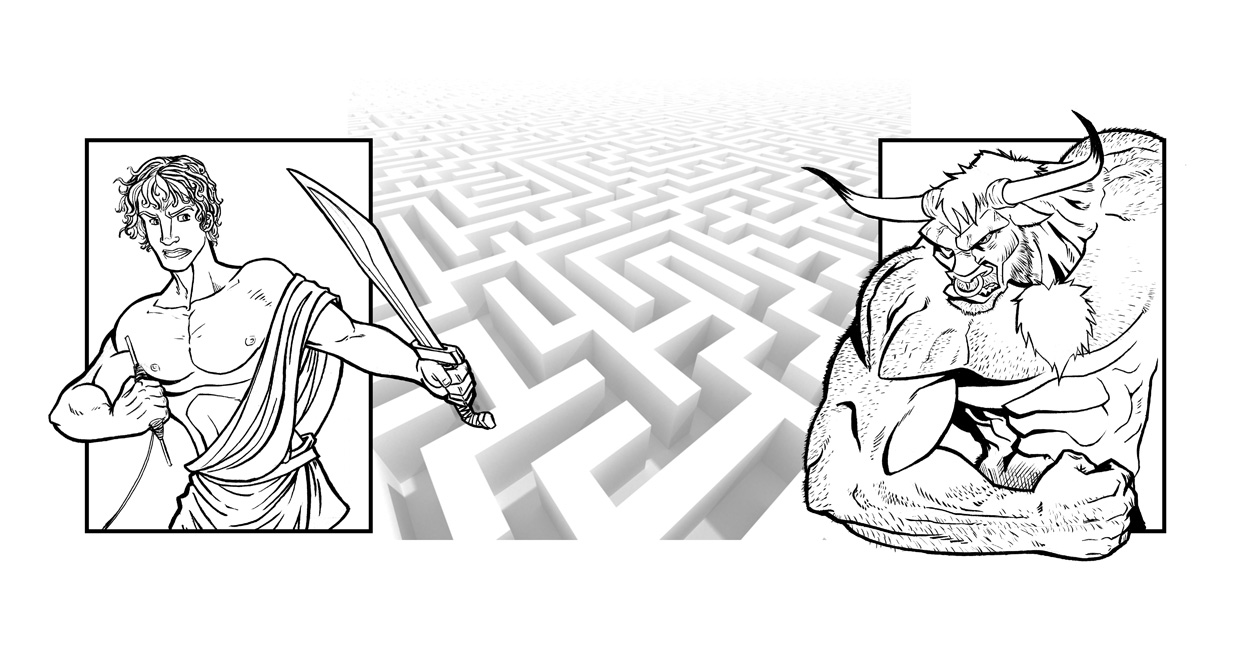
\includegraphics[height=5cm]{./images/teseo.jpg}
\end{center}


  \end{frame}



\end{document}
